% SE-INTEL Lite - Phase 2 paper SKELETON (IEEEtran, two-column).
% The course requires the text to be written by the group members in their own words.
% This file contains only structure, required-content notes (% NOTE lines, invisible in the PDF),
% and tables/figures generated from results/ by scripts/make_paper_assets.py. Replace every
% \todo{} with your own writing. Every number must come from results/.
\documentclass[conference]{IEEEtran}
\usepackage{graphicx,booktabs,amsmath,url,xcolor}
\usepackage[hidelinks]{hyperref}
\newcommand{\todo}[1]{\textcolor{red}{[TODO: #1]}}
\graphicspath{{../results/figures/}}

\begin{document}
\title{\todo{Paper title}}
\author{
\IEEEauthorblockN{Abdullah Bin Nasir (23I-0803)}
\IEEEauthorblockA{\todo{email}}
\and
\IEEEauthorblockN{Marvan Shahid (23I-0800)}
\IEEEauthorblockA{i230800@isb.nu.edu.pk}
\and
\IEEEauthorblockN{Project code: G3-13}
\IEEEauthorblockA{AI4015 Agentic AI, FAST-NUCES Islamabad}
}
\maketitle

\begin{abstract}
% NOTE 150-250 words: problem, approach, main quantitative results (from results/), contribution.
\todo{Abstract}
\end{abstract}

\section{Introduction}
% NOTE motivation; the three research gaps; research questions RQ1-RQ3; short list of contributions.
\todo{Introduction}

\section{Related Work}
% NOTE synthesis of the Phase 1 review: graph agents for code [LocAgent, RepoGraph, CodexGraph, CGM, OrcaLoca],
% repository QA [SWE-QA], code smells/quality, defect/vulnerability prediction, explainability, calibration.
% Position against the base paper. Target 25-30 references overall (see refs.bib).
\todo{Related work}

\section{Problem Formulation}
% NOTE define inputs (repository at commit c, question q), outputs (answer + evidence ids; hotspot ranking;
% p(file receives a bug fix in window W)), and the hypotheses H1-H3 exactly as pre-registered in Phase 1.
\todo{Problem formulation}

\section{Proposed System}
% NOTE architecture figure (docs/architecture.md), agent loop and state, the six tools,
% the component for each gap and its ablation switch (Table in docs/architecture.md).
\todo{System description}

\section{Experimental Setup}
% NOTE data (Table~\ref{tab:data}), SWE-QA version and dev/test split (20/172), time-based splits,
% baselines B0/B1/B2, model names and settings, 3 runs, implementation details.
\begin{table}[t]\centering\caption{Evaluation repositories at their pinned commits}\label{tab:data}
\resizebox{\columnwidth}{!}{\begin{tabular}{lrrrrrc}
\toprule
Repo & Files & Funcs & Edges & Commits & Fix commits & Test window \\
\midrule
requests & 36 & 669 & 1747 & 4768 & 542 & 2016--2025 \\
flask & 83 & 1397 & 3498 & 3753 & 459 & 2020--2025 \\
xarray & 233 & 7847 & 25537 & 5593 & 926 & 2023--2025 \\
pytest & 260 & 5654 & 15425 & 12373 & 2288 & 2020--2025 \\
\bottomrule
\end{tabular}
}\end{table}
\todo{Experimental setup}

\section{Evaluation Methodology}
% NOTE SWE-QA judge rubric (5x20), multi-hop label, P@10/nDCG@10, AUC/Brier/ECE, bootstrap,
% Wilcoxon, how the base-paper comparison is made (B2 reproduced by us).
\todo{Evaluation methodology}

\section{Results}
\subsection{Gap 1: Repository question answering}
\todo{Gap 1 results - run experiments/run\_qa.py and analyze\_qa.py first}
\subsection{Gap 2: Graph-aware quality hotspots}
\begin{table}[t]\centering\caption{Gap 2: P@10 per repository and mean P@10 / nDCG@10 on the test window}\label{tab:gap2}
\resizebox{\columnwidth}{!}{\begin{tabular}{lcccccc}
\toprule
Ranking & req. & flask & xarray & pytest & P@10 & nDCG@10 \\
\midrule
LOC (baseline) & 0.7 & 0.8 & 1.0 & 1.0 & 0.875 & 0.851 \\
Complexity only & 0.6 & 0.8 & 1.0 & 1.0 & 0.850 & 0.848 \\
Graph only & 0.6 & 0.8 & 1.0 & 1.0 & 0.850 & 0.767 \\
Hotspot (ours) & 0.6 & 0.8 & 1.0 & 1.0 & 0.850 & 0.862 \\
Churn & 0.6 & 0.8 & 1.0 & 1.0 & 0.850 & 0.861 \\
Churn $\times$ CC & 0.6 & 0.8 & 1.0 & 1.0 & 0.850 & 0.869 \\
\bottomrule
\end{tabular}
}\end{table}
\begin{figure}[t]\centering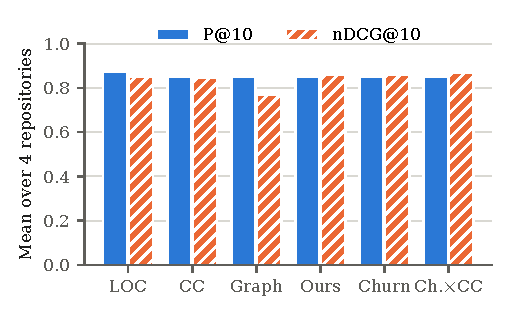
\includegraphics[width=\columnwidth]{gap2_rankings}
\caption{Gap 2: mean ranking quality over the four repositories.}\label{fig:gap2}\end{figure}
\todo{Gap 2 results, refer to Table~\ref{tab:gap2} and Fig.~\ref{fig:gap2}}
\subsection{Gap 3: Calibrated risk}
\begin{table}[t]\centering\caption{Gap 3: AUC / Brier / ECE per repository on the test period}\label{tab:gap3}
\resizebox{\columnwidth}{!}{\begin{tabular}{lcccc}
\toprule
Model & requests & flask & xarray & pytest \\
\midrule
Static only & 0.63 / 0.252 / 0.25 & 0.72 / 0.231 / 0.24 & 0.84 / 0.176 / 0.12 & 0.90 / 0.125 / 0.14 \\
Metrics only (static+change) & 0.70 / 0.278 / 0.28 & 0.62 / 0.243 / 0.17 & 0.80 / 0.182 / 0.14 & 0.92 / 0.114 / 0.12 \\
Full (ours) & 0.69 / 0.267 / 0.29 & 0.61 / 0.242 / 0.24 & 0.80 / 0.193 / 0.15 & 0.87 / 0.127 / 0.18 \\
Full, no calibration & 0.69 / 0.284 / 0.31 & 0.61 / 0.256 / 0.30 & 0.80 / 0.204 / 0.18 & 0.87 / 0.131 / 0.19 \\
\bottomrule
\end{tabular}
}\end{table}
\begin{figure}[t]\centering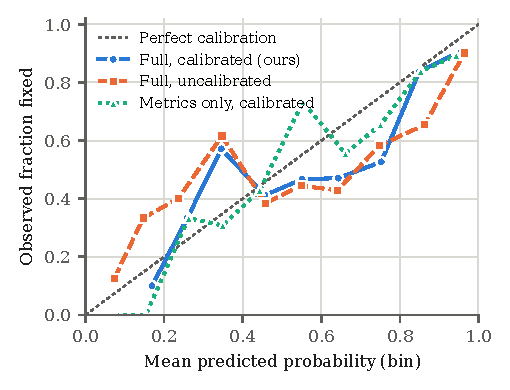
\includegraphics[width=0.9\columnwidth]{gap3_reliability}
\caption{Gap 3: reliability diagram on the pooled test files.}\label{fig:gap3}\end{figure}
\todo{Gap 3 results, refer to Table~\ref{tab:gap3} and Fig.~\ref{fig:gap3}}
\subsection{Gap-resolution table}
\begin{table*}[t]\centering\caption{Gap-resolution summary}\label{tab:gaps}
\resizebox{\textwidth}{!}{\begin{tabular}{p{1.6cm}p{2.6cm}p{2.0cm}p{2.8cm}p{3.2cm}p{1.2cm}}
\toprule
Gap & Method / component & Metric & Base paper result & Our result & Addressed? \\
\midrule
Gap 1: repository QA with typed multi-hop graph agent & ReAct graph agent + QA protocol + citation verifier (P) & SWE-QA overall /100 & not run & not run (needs LLM API key; see README) & - \\ \midrule
Gap 2: quality signals tied to the dependency graph & RunQuality/GetHotspots + hotspot = z(CC) + 0.25z(fan-in) + 0.25z(fan-out) & P@10 / nDCG@10 vs later bug-fix files (test window) & LocAgent: no quality signal. LOC ranking: 0.875 / 0.851 & 0.850 / 0.862 (-2.5 pp P@10 vs LOC) & Not \\ \midrule
Gap 3: calibrated, graph-aware risk under a time-based split & GetRisk: logistic regression (static + change + graph) + Platt calibration & Brier / ECE / ROC AUC on later period (mean of 4 repos) & LocAgent: no risk estimate. Metrics-only model: Brier 0.2043, AUC 0.762 & Brier 0.2072, ECE 0.218, AUC 0.744; Brier better on 2/4 repos & Partially \\ \midrule
\bottomrule
\end{tabular}
}\end{table*}

\section{Ablation and Comparative Analysis}
% NOTE results/e5_ablation_test.csv, results/gap3 (A4 no graph, A5 no calibration), results/e6_efficiency_test.csv
\todo{Ablation and efficiency}

\section{Failure Analysis}
% NOTE results/failures/categories_test.json: categories with frequencies, 2 success + 2 failure trajectories.
\todo{Failure analysis}

\section{Limitations and Threats to Validity}
% NOTE see README "honest reading" and docs/devlog.md entries 6-8: saturated long windows, small file
% populations, keyword label noise, collinear explanations, static-analysis blind spots, judge bias.
\todo{Limitations}

\section{Conclusion}
\todo{Conclusion and future work}

\bibliographystyle{IEEEtran}
\bibliography{refs}
\end{document}
